\documentclass[./A14_Report.tex]{subfiles}

\begin{document}
\chapter{Implementation}

\section{Design constraints}
The following constraints were considered during the implementation process to
simplify the design:
\begin{itemize}
    \item The images are assumed to be square in shape
    \item The dimensions of the image are assumed to be exact powers of two
    \item The images are in greyscale
    \item The entropy encoder has been left out of our implementation for simplicity
\end{itemize}

\section{The ``Transformer'' block}

An external C library for performing wavelet transforms is used. It is fully
open source. We have modified the library, to suit it to our needs
\cite{rpwavelib}. The interface is straightforward, providing access to each
sub-band for a particular level. A snippet of the access is given below.

\begin{code}
    \begin{minted}[bgcolor=codebg]{c}
    // Assume ROWS and COLS to be the dimensions of the image
    wave_object obj;
    wt2_object wt;
    double *inp, *wavecoeffs, *cLL;
    int N = ROWS*COLS;
    int ir, ic;
    char *name = "db2";
    obj = wave_init(name); // Initialize the wavelet
    inp = (double*) calloc(N, sizeof(double));
    int J = 1; // decomposition level
    wt = wt2_init(obj, "dwt", ROWS, COLS, J);
    // Assume pix_arr is a row-major array of 8-bit pixel values
    for (int i = 0; i < ROWS; ++i) {
        for (int k = 0; k < COLS; ++k) {
            inp[i*COLS + k] = (double) pix_arr[i*COLS + k];
        }
    }
    wavecoeffs = dwt2(wt, inp);
    cLL = getWT2Coeffs(wt, wavecoeffs, 1, "A", &ir, &ic);
    \end{minted}
    \caption{\texttt{wavelib} LL sub-band extraction example \cite{libezw}}
    \label{code:wavelibex}
\end{code}

\pagebreak

The sub-band coefficients are stored in a hierarchical tree-like structure for
easy access of coefficients. It is shown in the figure below.

\begin{figure}[H]
    \centering
    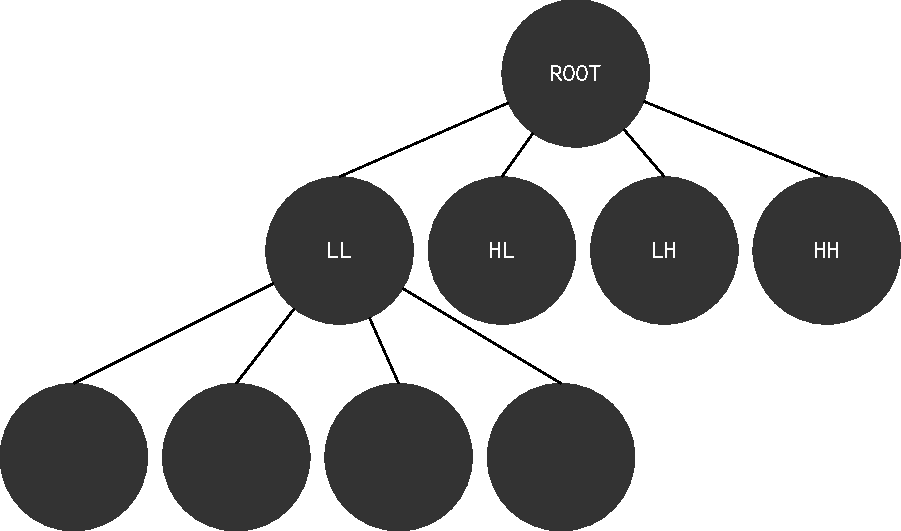
\includegraphics{sbtree.pdf}
    \caption{Sub-band tree \cite{libezw}}
    \label{fig:sbtreediag}
\end{figure}

The main root node is treated specially and does not contain any coefficients.
Every other node contains a row-major array of it's coefficients. It must also
be observed that only the \textit{LL} sub-bands have children. This is because
only the \textit{LL} sub-band is sub-divided further in our procedure.
\begin{code}
\begin{minted}[bgcolor=codebg]{c}
enum sb_type {
    LL,
    HL,
    LH,
    HH,
    ROOT
};
typedef struct SBtree_node {
    struct SBtree_node *ll;
    struct SBtree_node *hl;
    struct SBtree_node *lh;
    struct SBtree_node *hh;
    double *coeffs;
    enum sb_type type;
} SBtree_node;
\end{minted}
\caption{\texttt{C struct} representation of the tree shown in figure \ref{fig:sbtreediag} \cite{libezw}}
    \label{code:sbtreedef}
\end{code}

\section{The ``Quantizer'' block}
This block deals with the approximation and labelling of the coefficients as
one of four \textit{significance values}, to construct what is called a
\textit{significance map}. The significance map is also modelled as a tree
whose nodes contain the coefficients and all associated information. If we move
deeper into the tree, the level of decomposition \textbf{decreases}. Another
key point about the tree is that the first node (the \textit{LL} coefficient of
the highest level of decomposition) has only 3 children, while all others have
four. % add a reference to Skanda's hierarchy image from before to show the relationship between each level of nodes

\begin{figure}[H]
    \centering
    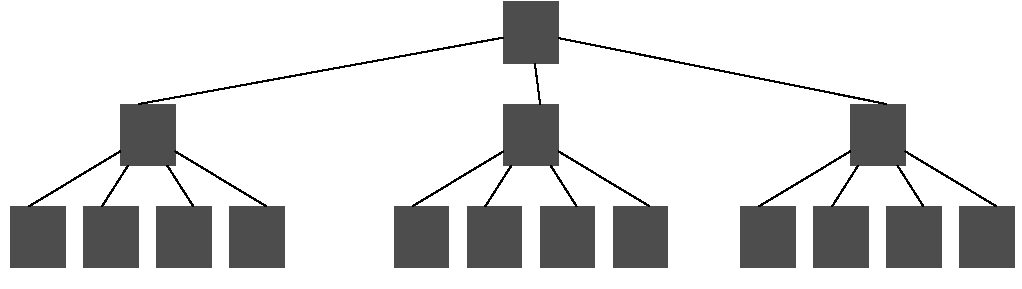
\includegraphics{smap.pdf}
    \caption{Significance map tree \cite{libezw}}
    \label{fig:smaptreediag}
\end{figure}

\begin{code}
\begin{minted}[bgcolor=codebg]{c}
enum smap_symbol { // significance map value
    SP = 0, // Significant Positive
    SN = 1, // Significant Negative
    IZ = 2, // Isolated Zero
    ZR = 3, // Zerotree Root
    U = -1 // Unitialized
};
typedef struct Smap_tree_node {
    double coeff;
    struct Smap_tree_node *parent;
    struct Smap_tree_node *children[4];
    char isroot : 1;
    enum smap_symbol type;
    unsigned char not_available;
} Smap_tree_node;
\end{minted}
\caption{\texttt{C struct} representation of the tree shown in figure \ref{fig:smaptreediag} \cite{libezw}}
    \label{code:sbtreedef}
\end{code}

\subsection{The algorithms}
The algorithm used to assign the significance map values to the respective
coefficients are split into two steps or ``passes'', the \textit{dominant pass}
and the \textit{subordinate pass} that happen one after the other \cite{shap1993}. Each set of
passes depends on a threshold value, with which coefficients are compared with
to decide what value they are mapped to.
\par
\textbf{PTO}

\begin{algorithm}[H]
    \caption{Dominant pass}
    \label{alg:dompass}
    \begin{algorithmic}
        \Require $smap\_tree\_root$ \Comment{Root of a significance map tree}
        \Require $threshold \in \mathbb{Z}^+$
        \State $node \gets \text{NULL}$
        % \State $threshold \gets 2^{\lfloor\log_2{MAX(coefficients)}\rfloor}$\\
        \ForAll{$node \in \text{level order of } smap\_tree\_root$}
            \State $check\_descendants(node, threshold)$
            \If{node is SP or SN or IZ}
                \State $dominant\_list \gets (dominant\_list, current\_node)$
            \ElsIf{node is ZR}
                \If{parent of node is not ZR or node is the root}
                    \State $dominant\_list \gets (dominant\_list, current\_node)$
                \EndIf
            \EndIf
        \EndFor
    \end{algorithmic}
\end{algorithm}

During the dominant pass, nodes in the tree (scanned breadth-first to get a
Morton scan) are compared with the current threshold, and assigned an
appropriate symbol. There are 4 possible symbols \cite{valezw1999}:\\

\begin{table}[H]
    \centering
    \begin{tabular}{|c|c|}
        \hline
        \textbf{Symbol} & \textbf{Binary Representation}\\
        \hline
        Significant Positive (SP) & $00$\\
        Significant Negative (SN) & $01$\\
        Isolated Zero (IZ) & $10$\\
        Zerotree Root (ZR) & $11$\\
        \hline
    \end{tabular}
    \caption{Quantization symbols}
    \label{tab:qsymbs}
\end{table}

This assignment is handled by the \mintinline{c}{check_descendants()} routine in
algorithm \ref{alg:dompass}. Once that is done, the significant nodes are put
in a list and returned to be used in the subordinate pass.

\begin{algorithm}[H]
    \caption{Subordinate pass}
    \label{alg:subpass}
    \begin{algorithmic}
        \Require $dominant\_list$
        \Require $threshold \in \mathbb{Z}^+$
        \State $subordinate\_list \gets \text{NULL}$
        \State $node \gets \text{NULL}$
        \ForAll{$node \in dominant\_list$}
            \State coeff $\gets$ coefficient of node
            \If{node is SP or SN}
                \If{$\lvert \text{coeff} \rvert > 1.5 \cdot t$}
                    \State Append a $1$ to $subordinate\_list$
                \Else
                    \State Append a $0$ to $subordinate\_list$
                \EndIf
            \Else
                \State Append a $0$ to $subordinate\_list$
            \EndIf
        \EndFor
    \end{algorithmic}
\end{algorithm}

In the subordinate pass, a refinement bit is added to help reconstruct the
coefficient when decoding. This also contributes to the quantization process,
along with the dominant pass. In this case, a $1$ is coded if the absolute
value of the coefficient of the node is greater than $1.5$ times the current
threshold, and a $0$ otherwise. These bits are filled in to a list and returned
for use later.

\begin{algorithm}[H]
    \caption{EZW Compression}
    \label{alg:ezw}
    \begin{algorithmic}
        \Require $smap\_tree\_root$ \Comment{Root of a significance map tree}
        \Require $min\_threshold \ge 0$
        \State $node \gets \text{NULL}$
        \State $threshold \gets 2^{\lfloor\log_2{MAX(\text{coefficients of } smap\_tree\_root)}\rfloor}$
        \While{$threshold > min\_threshold$}
            \State $dominant\_list \gets$ dominant\_pass(smap\_tree\_root, threshold)
            \State $subordinate\_list \gets subordinate\_pass(dominant\_list, threshold)$
            \State Write data to file
            \State $threshold \gets threshold/2$
        \EndWhile
    \end{algorithmic}
\end{algorithm}

Finally, in the actual EZW algorithm, the initial threshold for a given set of
coefficients is calculated as the power of $2$ that is nearest to the largest
coefficient. Once this is done, the dominant and subordinate passes are called
in succession, while halving the threshold after each iteration. This increases
the amount of precision in the data every iteration. This is the successive
approximation quantization process, where the step-size of the quantizer is
decreased every iteration \cite{shap1993}. The information that is written to a
file must include the dominant and subordinate lists for each pass for correct
reconstruction. This information may be compressed even more using entropy
coding techniques.

\begin{algorithm}[H]
    \caption{EZW Decompression}
    \label{alg:ezwdecomp}
    \begin{algorithmic}
        \Require $compressed\_file$
        \State $dominant\_list \gets \text{NULL}$
        \State $subordinate\_list \gets \text{NULL}$
        \ForAll{$dominant\_list, subordinate\_list$}
            \State Approximate coefficients in $dominant\_list$
            \State Refine respective coefficients using $subordinate\_list$
            \State Write data to file
        \EndFor
    \end{algorithmic}
\end{algorithm}

The decompression process is, by nature, the reverse of the compression
process. The steps involved in the approximation and refinement process are as
follows:
\begin{enumerate}
    \item{Check the current symbol}
    \item{If significant, assign it the value $1.5 \times T_i$}
        \begin{enumerate}
            \item{If the refinement bit is set, add $\frac{T_i}{4}$ to the
                value set before, otherwise, subtract it.}
            \item{If the symbol is labelled negative, multiply with $-1$}
        \end{enumerate}
    \item{Read next symbol}
\end{enumerate}

The below code snippet shows how it is implemented.

\begin{code}
\begin{minted}[bgcolor=codebg]{c}
switch(symbol) {
    case SP:
        {
            if(lsb) {
                curr_smap->coeff = (1.5*curr_threshold) + (curr_threshold/4.0);
            }
            else {
                curr_smap->coeff = (1.5*curr_threshold) - (curr_threshold/4.0);
            }
            curr_smap->not_available = 1;
            break;
        }
    case SN:
        {
            if(lsb) {
                curr_smap->coeff = -((1.5*curr_threshold) + (curr_threshold/4.0));
            }
            else {
                curr_smap->coeff = -((1.5*curr_threshold) - (curr_threshold/4.0));
            }
            curr_smap->not_available = 1;
            break;
        }
    default:
        {
            curr_smap->coeff = 0.0;
            break;
        }
}
\end{minted}
\caption{Approximation of coefficients \cite{libezw}}
    \label{code:sbtreedef}
\end{code}
\vspace{0.5cm}

Consider the example shown in figure \ref{fig:exa}
\cite{sayood_datac}:

\begin{figure}[H]
    \begin{subfigure}[b]{0.5\textwidth}
        \centering
        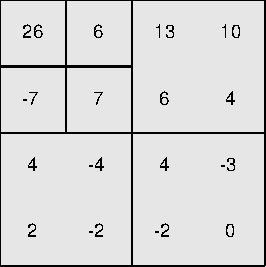
\includegraphics[width=0.5\textwidth]{example1.pdf}
        \caption{Original}
        \label{fig:exa}
    \end{subfigure}
    \hfill
    \begin{subfigure}[b]{0.5\textwidth}
        \centering
        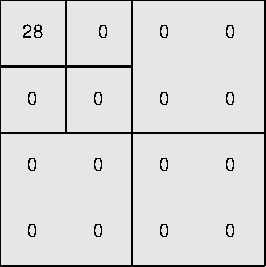
\includegraphics[width=0.5\textwidth]{example2.pdf}
        \caption{Reconstruction for first set of passes}
        \label{fig:exb}
    \end{subfigure}
    \caption{Example decomposition}
    \label{fig:ex}
\end{figure}

\begin{displaymath}
    T_0 = 2^{\lfloor\log_2{26}\rfloor} = 16
\end{displaymath}
\begin{displaymath}
    D = \{SP, ZR, ZR, ZR\}\\
\end{displaymath}
\begin{displaymath}
    S = \{1\}\\
\end{displaymath}

After the first round of reconstruction, we will get the decomposition shown in
figure \ref{fig:exb}. The value $28$ is found as follows:
\begin{displaymath}
    T_0 = 16
\end{displaymath}
\begin{displaymath}
    Approx = 1.5 \times T_0 = 24
\end{displaymath}
\begin{displaymath}
    Refined = 24 + \frac{T_0}{4} = 28
\end{displaymath}
This process is repeated until a limit (can be decided by user), as shown in
algorithm \ref{alg:ezw} to increase the accuracy of the reconstruction.

\section{File format}
The output file consists of the symbols extracted during the dominant pass,
along with the refinement bits. The threshold value of each iteration and the
dimensions of the image are also part of the file. The binary file consists of
a \textit{main-header} and several \textit{mini-headers}, followed by the data.
The symbols are packed 2 at a time into bytes to save space. Entropy encoding
could have helped save even more space at this stage. The first byte of the
file is the power of $2$ that represents the dimensions of the image. So, if we
have a $d \times d$ image, the first byte will have the value $\log_2{d}$.  The
packet format is specified in figure \ref{fig:packet}. There will be one packet
for every iteration of the algorithm. Assume there are $k$ symbols to be
written for the current iteration. Then-
\begin{displaymath}
    t = \log_2{T_i}
\end{displaymath}
\begin{displaymath}
    n = \frac{k}{2} + (k \bmod 2)
\end{displaymath}

\begin{figure}[H]
    \centering
    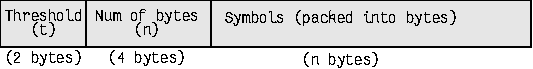
\includegraphics{packet.pdf}
    \caption{Packet format}
    \label{fig:packet}
\end{figure}

When reading the file, the information can be extracted by using bit-masks and
clever bitwise operations.

\end{document}
